
\definecolor{codegreen}{rgb}{0,0.6,0}
\definecolor{codegray}{rgb}{0.5,0.5,0.5}
\definecolor{codepurple}{rgb}{0.58,0,0.82}
\definecolor{backcolour}{rgb}{0.95,0.95,0.92}

\lstdefinestyle{mystyle}{
	backgroundcolor=\color{backcolour},   
	commentstyle=\color{codegreen},
	keywordstyle=\color{magenta},
	numberstyle=\tiny\color{codegray},
	stringstyle=\color{codepurple},
	basicstyle=\ttfamily\footnotesize,
	breakatwhitespace=false,         
	breaklines=true,                 
	captionpos=b,                    
	keepspaces=true,                 
	numbers=left,                    
	numbersep=5pt,                  
	showspaces=false,                
	showstringspaces=false,
	showtabs=false,                  
	tabsize=2
}

In this section, we address the problem presented in Section \ref{sec:PBS}. To do so, we begin by generating synthetic data using a PRNG. Based on this data, we construct a polynomial regression model using OLS.

\noindent Next, we apply a resampling technique to create multiple datasets derived from the original synthetic dataset. For each resampled dataset, a separate polynomial regression model is trained. Finally, we evaluate and compare the performance of these models using various metrics, including MBE and RMSE. The code is based on module 4 from the course 'Anvendt statistik' \cite{ASTA}, with assistance from AI 

\subsection{Setting Up the Models}
To understand how assumption violations affect classical polynomial regression, we begin by generating synthetic data using a random number generator, as shown in \autoref{code1}. First, four independent variables are created, each normally distributed with known standard deviations. Then, the dependent variable is generated as a function of these four independent variables. This synthetic dataset initially satisfies all the assumptions required for ordinary least squares regression. Next, an error term is added that scales with the dependent variable. This introduces heteroscedasticity meaning the error variance is no longer constant thereby violating the assumption of homoscedasticity. This step is done deliberately to ensure that this is the only assumption being violated, so any observed effects on the model can be attributed specifically to this violation.
\\\\


\lstinputlisting[language=R, caption=Datageneration and adding hetroscedasety,label=code1, firstline=8, lastline=25]{kode/sammenligning2.R}


\noindent The dataset is then in \autoref{code2} line 2-6 split into training and test sets, with $80\%$ used for training and the remaining $20\%$ for testing. A standard linear polynomial regression model is fitted to the training data on line 8. The standard error, and confidence intervals for the coefficients are calculated on line 11 - 5 the $R^2$ is calculeted on line 18 and  the mean bias error and root mean squared error calculated are useing the testdata on line 21- 25 all this is to evaluate the model's performance.
\\\\
\lstinputlisting[language=R, caption=traning/test data and OLS,label=code2, firstline=27, lastline=53]{kode/sammenligning2.R}


\noindent Following this,the amount of resamples for the bootstrap are set at 10000 and the function for the coefficients are defined in line 1-9 and a bootstrap is then performed by resampling the training data in line 11-30. For each resampled dateset, a linear polynomial model is fitted. The $R^2$, coefficients and the predictions on the test data. These predictions are then used to compute the mean bias error and RMSE and the coefficients are used the calculated the standard error and confidence intervals of the coefficients for the bootstrap models.
\\\\\\\\\\\\

\lstinputlisting[language=R, caption=Bootstrap, label=code3, firstline=54, lastline=97]{kode/sammenligning2.R}


\subsection{Results}
Comparing the results of the two models shown in Table 2, the Mean Bias Error, MBE, of the OLS model is -546.4660, indicating that it tends to underpredict the actual values. In contrast, the bootstrap model has an MBE of 17.7164, suggesting only a slight over-prediction. The smaller absolute bias of the bootstrap model indicates improved accuracy. This is further supported by the Root Mean Square Error, RMSE, where the OLS model scores 1884.5830 compared to the bootstrap model’s 1350.7740. This substantial difference reinforces the conclusion that the bootstrap model provides more accurate predictions.
\\\\
When comparing the standard errors of the estimated coefficients, the OLS model appears to have lower standard errors. However, it is important to note that these may not be reliable due to the violation of the homoscedasticity assumption. In such cases, the standard errors from OLS can be misleading. In contrast, the bootstrap standard errors are derived from the empirical distribution of the data and are therefore more representative of the true variability. As a result, the confidence intervals produced by the OLS model may not be trustworthy, while those from the bootstrap model better reflect the uncertainty in the estimates showing a false sense of predictability. Overall, the bootstrap approach demonstrates superior predictive performance and more robust inference under assumption violations.
\\\\
the $R^2$ of the OLS is 0.8552 compering it to the mean of the bootstraps $R^2$ that is 0.7891 and median that is 0.8688. it is clear that there are a big differences this difference indicates a skewed  $R^2$ distribution this is truther shown in \autoref{fig:5} where it is clear that the $R^2$ distribution is heavily skewed. this also explains the 95\% confide interval of the  $R^2$ distribution being $[ 0.2468 ,  0.9656 ] $ witch is extremely wide


\begin{table}[h!]
	\centering
	\caption{Comparison of OLS and Bootstrap model}
	\begin{tabular}{lcc}
		\hline
		& \textbf{OLS} & \textbf{Bootstrap} \\
		\hline
		\textbf{MBE} & -546.4660 & 17.7164 \\
		\textbf{RMSE} & 1884.5830 & 1350.7740 \\
		\textbf{R-squared} & 0.8552 & Median: 0.8688 Mean: 0.7891  \\
		& & 95\% CI [ 0.2468 ,  0.9656 ] \\
		\hline
		\textbf{Std. Error} \\
		\hline
		Intercept & 475.7736 & 534.8255 \\
		$I(x1^2)$ & 3.5947e-04 & 8.4177e-04 \\
		$I(x2^3)$ & 3.7720e-08 & 1.2377e-07 \\
		$I(x3^4)$ & 4.6861e-13 & 3.3556e-10 \\
		$I(x4^5)$ & 7.4733e-15 & 1.4069e-13 \\
		\hline
		\textbf{Coefficient (95\% CI)} \\
		\hline
		Intercept & [2835.399 , 4767.143] & [2424.484 , 4508.749] \\
		$I(x1^2)$ & [1.2481e-04 , 1.5844e-03] & [6.0011e-04 , 3.2840e-03] \\
		$I(x2^3)$ & [-1.3172e-07 , 2.1432e-08] & [-3.2404e-07 , 8.1277e-08] \\
		$I(x3^4)$ & [2.1146e-12 , 4.0173e-12] & [2.6966e-12 , 7.9974e-10] \\
		$I(x4^5)$ & [-1.0574e-13 , -7.5394e-14] & [-1.3206e-13 , 2.5471e-13] \\
		\hline
	\end{tabular}
\end{table}


\begin{figure}[h]
	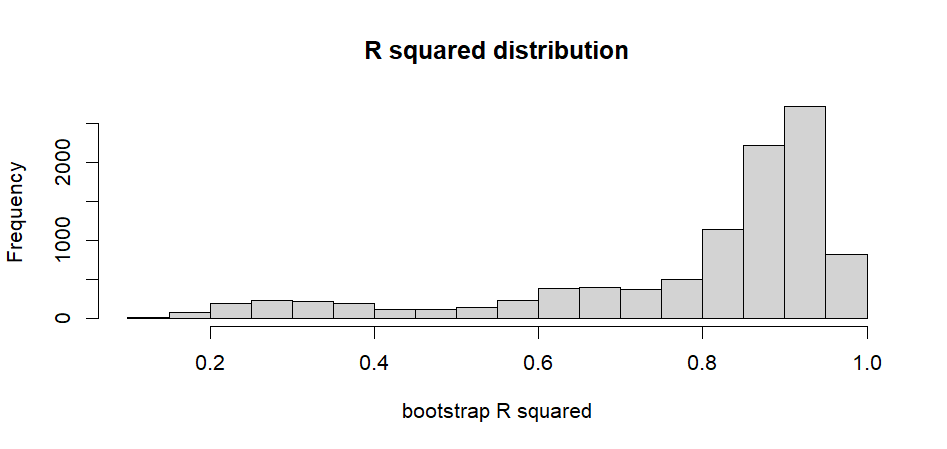
\includegraphics[width=\linewidth]{billder/R^2v2.png}
	\caption{$R^2$ distribution}
	\label{fig:5}
\end{figure}

